% LaTeX file for resume
% This file uses the resume document class (res.cls)

\documentclass{resumecls}
\usepackage{ctex}
\usepackage{cmap}
\usepackage{url}
\usepackage{calc}
% \usepackage[top=10mm,bottom=10mm,left=12.5mm,right=12.5mm]{geometry}
\usepackage{hyperref}
\usepackage{tabularx}	
\usepackage{verbatim}
\usepackage{multicol}
\usepackage{graphicx}
\usepackage{multirow}
\usepackage{ulem}
\usepackage{wallpaper}

\hypersetup{colorlinks,breaklinks,
			urlcolor=blue,
			linkcolor=blue}
\newcommand{\Photo}{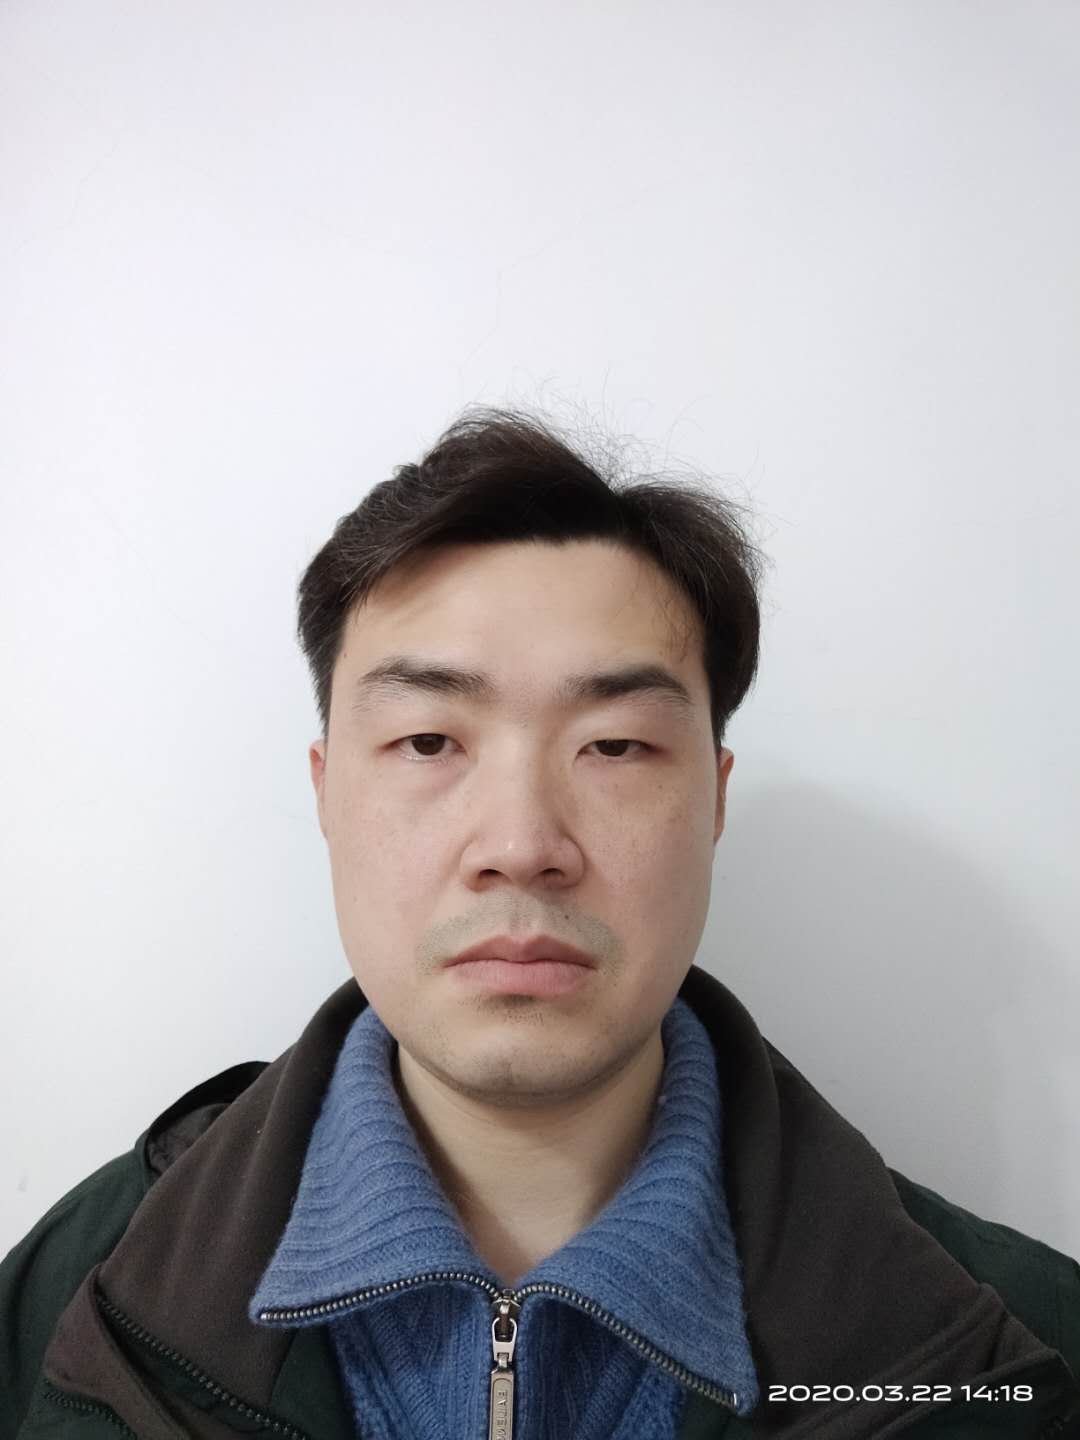
\includegraphics[origin=lt,width=20mm]{face20200322141953.jpg}}
\newlength{\DateWidth}\settowidth{\DateWidth}{\bf{2001.01~--~2001.01}}
\newlength{\TableWidth}\setlength{\TableWidth}{\textwidth}

\newcommand{\WorkExperience}[5]{
    \noindent
    %\hspace{-0.5cm}
    \begin{tabularx}{\TableWidth}{>{\hsize=0.382\hsize}XX}
    \textbf{#1}  & \textbf{#2}\\
    部门         & #3\\
    任职         & #4\\
    描述         & #5
    \end{tabularx} \\
}

\newcommand{\ProjectExperience}[4]{
    \noindent
    %\hspace{-0.5cm}
    \addtocounter{Project}{1}
    \begin{tabularx}{\TableWidth}{>{\hsize=0.382\hsize}XX}
    \multicolumn{2}{l}{\bf \Roman{Project}.~#1}\\
    \it{项目描述}              & #3\\
    \it{职责范围}              & #4\\
    \it{相关技术}    			 & #2\\
    \end{tabularx}\\
}

\newlength{\PhotoWidth}\settowidth{\PhotoWidth}{\Photo}
\renewcommand{\heading}[1]{
    \colorbox{heading}{
        \parbox{.98\textwidth}{
            \bfseries\zihao{4}#1
        }
    } \\
}

\begin{document}
\pagenumbering{arabic}
\rfoot{\thepage}
%\TileSquareWallPaper{2}{wallpaper.pdf}
\name{张甡华\\}     % the \\[12pt] adds a blank
				        % line after name


\leftfooter{最后更新: \today}


\section{自我介绍}
我叫张甡华,我从历史中来,终将变成历史。
我入行IT比较早,有非常丰富的工作经历、经验、阅读量以及精彩故事。
具有踏实肯干实事求是的作风。
不自信是我最主要的性格特征。
不自信到什么地步呢?
不自信到,不向任何人保证我说的任何一句话绝对真实。
我有良好的辨证思维、底线思维、系统思维习惯。敢于提出建设性、非建设性、现实或空想的意见。
我是讲信用的,答应办的事情就会去办,办好办坏都会出个结果。就历史来看,办事成功率不低于70\%。
我希望朋友们在这个基础上来认识我这个人。不能指望通过本简历全面认识我本人。



\section{基本信息}
    \noindent
    \begin{tabularx}{\TableWidth-10mm}{XXp{\PhotoWidth}X}
        1982-09-13 生于上海         & 工作年限 $>$ 14年             & \multirow{4}{\PhotoWidth}{\Photo}\\
        \multicolumn{2}{l}{\textbf{职业} 软件设计师, 软件工程师}   & \\
        \multicolumn{2}{l}{\textbf{email} \href{mailto:zhang1.61803398@foxmail.com}{zhang1.61803398@foxmail.com}} & \\
        \multicolumn{2}{l}{\textbf{Tel} 138 1824 8880 (Mobile)}  & \\
    \end{tabularx}



\section{教育背景}
    \noindent
    \begin{tabularx}{\TableWidth}{>{\hsize=0.382\hsize}XX}
    \bf{2008.9~--~2011.10}  &  中央广播电视大学(本科),计算机科学与技术。\par
                               核心课程包括《离散数学》、《计算机组成原理》、《软件工程》、《C语言程
								序设计》、《数据结构》、《操作系统》、《数据库应用技术》、《计算机网络》
								等。\\
    \bf{2002.9~--~2005.07}  &  中央广播电视大学(专科),计算机实用技术。\par
                               核心课程包括《高等数学》、《线性代数》、《C语言程序设计》、《数据结
构》、《操作系统》、《数据库技术》、《VB程序设计》、《Java语言程序设
计》、《微机原理与汇编语言程序设计》、《专业英语》、《计算机辅助设计》
等。
    \end{tabularx} \\

\section{专业技能}
    \begin{multicols}{4}
    \begin{itemize}
      \item[]BASIC(VB)
      \item[]Pascal(Delphi)
      \item[]C\#(.NET)
      \item[]C/C++
      \item[]软件工程
      \item[]数学知识
      \item[]算法技术
      \item[]TCP/IP网络编程
      \item[]关系数据库
      \item[]Python
      \item[]linux
      \item[]Perl
      \item[]Git
      \item[]UNIX
      \item[]\TeX
      \item[]LISP
      \item[]HTML
      \item[]nginx
      \item[]samba
      \item[]fcgi
      \item[]Javascript
      \item[]node
      \item[]mongodb
    \end{itemize}
    \end{multicols}
\section{工作经验}
    \WorkExperience
        {2017.6~--~2019.11}
        {澳博汇融金融信息服务(上海)有限公司}
        {技术管理部}
        {IT主管}
        {提供从内网建设到贷后MIS软件开发的全栈服务。实现公司业务流程的系统化、信息化以及数据打通,
        为上层决策提供依据。}
        
    \WorkExperience
        {2016.1~--~2016.6}
        {上海敬一信息科技有限公司}
        {*}
        {项目助理、黑盒测试、白盒测试、缺陷管理}
        {为团队制定工作流程。结合公司实际业务推行实施gitlab工作流。}
        
    \WorkExperience
        {2014.8~--~2015.8}
        {Archermind}
        {Intel ICG、SSG、QCTV}
        {软件工程师}
        {Camera Automation Test Python脚本维护,Tools Develop.编写日志分析程序}

    \WorkExperience
        {2013.6~--~2014.8}
        {自由职业}
        {*}
        {自由开发者}
        {苹果APP开发,开发一款阅读软件。}

    \WorkExperience
        {2012.11~--~2013.6}
        {兴业银行}
        {卡中心信息科技部}
        {主任工程师、项目经理}
        {银行中间业务开发}

    \WorkExperience
        {2011.8~--~2012.9}
        {HiSoft(海辉软件)}
        {SH Embedded DEV, Intel McG PIV}
        {软件工程师}
        {Embedded Develop, Android Debug, Automation Tools Develop}

   \WorkExperience
       {2008.6~--~2011.07}
       {上海广电通信技术有限公司}
       {总师办实验室、显示通信分公司}
       {软件工程师}
       {雷达应用软件开发, 雷达数据分析与算法研究,雷达数据分析工具开发,LED应用软件开发。}
   \WorkExperience
       {2006.1 -- 2008.6}
       {华东师范大学科教仪器厂}
       {研发中心、网络部}
       {软件工程师}
       {网络应用程序开发,教学用程序开发,嵌入式开发}
   %\newpage
\section{项目经验}
    \newcounter{Project}
    \ProjectExperience
        {cosmos(非COSMOS区块链)网络实验}
        {Linux, node, mongodb, HTML, Javascript}
        {
        为贷后部门打造处理每日成千上万笔应收款的工具,并根据划扣和还款情况作大数据统计。
        }
        {提出者,参与者,实现者}
        
    \ProjectExperience
        {贷后系统}
        {Linux,samba,Nginx,FCGI,PERL,HTML,Javascript}
        {
        为贷后部门打造处理每日成千上万笔应收款的工具,并根据划扣和还款情况作大数据统计。
        }
        {全栈}
        
    \ProjectExperience
        {文件服务器搭建}
        {Linux,samba}
        {
        为公司搭建并管理可审计、分权限的文件服务器。
        }
        {需求听取、规划、实施}
        
    \ProjectExperience
        {数字化教学平台}
        {C\#.net, Javascript, GIT}
        {
        为团队制定软件开发的工作流。
        }
        {项目助理, 需求分析, 黑盒测试, 白盒测试}
\iftrue
    \ProjectExperience
        {联通快捷支付项目}
        {AIX, C,RPO*C, ORACLE,银联数据发卡系统接口、银行行业组态软件}
        {
        兴业银行联通快捷支付项目。包括:签约、签约撤销、快捷支付、退货、对
		账、自动资金清算、报表生成。
        }
        {项目经理、需求分析、程序设计、编码、测试}

    \ProjectExperience
        {信用卡积分管理系统}
        {AIX, C,RPO*C, ORACLE,银联数据发卡系统接口、银行行业组态软件}
        {
        兴业银行信用卡积分管理系统。包括:日交易数据导入、规则引擎、积分
		计算、批量调帐、对账。
        }
        {需求分析、程序设计、编码、测试}
\fi

    \ProjectExperience
        {Build-Server}
        {Linux,Python, XML}
        {
        一个Linux下软件环境的编译与发布平台。(Intel)
        }
        {需求分析、架构设计、编码}

    \ProjectExperience
        {Android Graphic Debug}
        {C, linux kernel, Android, OpenGL}
        {
        Ϊ为Andriod平台的移动设备Debug。(主要针对Graphic域)(Intel)}
        {Debug}

    \ProjectExperience
        {Andorid自动测试框架}
        {Python, MonkeyRunner}
        {为Andorid平台的移动设备构建一个自动化测试框架。(Intel)}
        {需求分析、编码、测试}

    \ProjectExperience
        {MTK手机平台下的YouKu客户端开发}
        {C, MTK}
        {领导团队将Android平台上的YouKu客户端移植到MTK手机平台上。}
        {需求分析、项目管理、编码、测试}

    \ProjectExperience
		{雷达视频数据切片、呈现、提取工具}
		{雷达,PPI,二进制文件分析,MATLAB}
		{用MATLAB构建一个工具,从雷达数据记录仪的保存的二进制文件中,提
取感兴趣的信息(一般为视频信息),将其保存为MATLAB文件,以供分
析研究。}
		{需求分析、数学建模、数据结构设计、架构设计、程序设计、编码、测试}
    \ProjectExperience
        {基于MATLAB的雷达算法仿真平台}
		{雷达,绘图算法,MATLAB}
		{
		用MATLAB构建一个雷达算法的仿真平台(在MATLAB上直接观察算法
		的效果),并省下DSP工程师编译与烧录的时间,提高研发效率。
		}
		{需求分析,数学建模,数据结构设计,架构设计,程序设计,编码,测试}

    \ProjectExperience
		{雷达终端死机问题的定位}
		{C++、BC3.1、DOS、debug技术}
		{XXX型雷达终端程序在一定情况下死机。利用各种调试手段分析程序异常
		退出原因。最终将问题定位于一个函数的一句语句上。}
		{分析、debug}

    \ProjectExperience
  		{雷达A/R型显示程序}
  		{雷达、C++、LINUX、Qtopia、数学建模}
  		{\ 一个雷达A/R型显示的应用程序。该程序目前在雷达产品上运行良好。
详见本人发表在《船用导航雷达》杂志第97期上题为《一种基于船用导航
雷达的A/R显示实现方法》的论文。}
  		{需求分析,数学建模,算法设计,架构设计,程序设计,编码,测试}

    \ProjectExperience
    	{LED静态模组测试卡}
        {C、C++、AVR单片机}
        {设计并实现一个嵌入式系统,根据LED模组的测试要求向欲测试模组发送
		测试信号。使其呈现一定测试图案。此项目申得一项实用新型专利。}
        {
        项目分硬件与软件两部分,本人主要负责软件部分。其中包括系统分析、
		算法设计、程序设计、编码、测试。
        }


    \ProjectExperience
        {交通光带屏光带地址表生成程序}
        {LISP、PYTHON、数学建模}
        {为了提高地址表制作的效率与准确性,便于地址表的维护与更新,本人自
		发性对此项工作进行技术改进。此项设计以本人为作者为公司申得软件著
		作权。专利号:\uline{2010SR039161}
        }
        {需求分析、数学建模、程序设计、编码、测试}

    \ProjectExperience
		{常州可变车道控制系统}
		{DELPHI、与LED控制卡的接口}
		{设计一个程序接受交警的操作来控制可变车道的通行指示灯。}
		{需求分析、程序设计、编码、现场设计修改、测试}

    \ProjectExperience
        {GPRS通信程序}
        {GPRS、GPRS供应商提供的API、DELPHI}
        {
        连通各GPRS设备与数据中心,使其进行数据传送。
        }
        {系统分析、编码}

    \ProjectExperience
        {NETM0动态链接库}
        {DLL、ActiveX DLL、COM、DELPHI、VC++}
        {
        对NETM0产品中动态链接库进行重新包装以供外单位(自动化所)使用,
		并编写DEMO程序使客户方程序员知晓如何使用此动态链接库。
        }
        {需求分析、接口设计、编码}

    \ProjectExperience
        {NETM1上位机软件进化}
        {Delphi}
        {
       	为NETM1这款LED屏控制软件作二次开发为其添置新功能。
        }
        {阅读代码、系统分析、编码}

    \ProjectExperience
        {手持式数据采集器}
        {C、C++、USB、嵌入式系统、ARM7、ucosII、液晶显示驱动、绘图算法}
        {
        对传感器数据进行采集、传输、显示和存储。
        }
        {嵌入式系统程序设计,算法设计、界面设计}

    \ProjectExperience
        {课程应用程序管理器}
        {VB,与时间相关的算法}
        {
        它让用户配置课程表和脚本,使得计算机能够在上不同课时自动打开与该
		课程相关教学环境。
        }
        {需求分析,体系结构设计,算法设计,所有程序设计与编码。}

    \ProjectExperience
        {学生机控制程序}
        {VC++, MFC, TCP/IP}
        {
        主机控制网络中学生机进程以及运行指定的程序。
        }
        {需求分析、体系结构设计、关键技术的程序设计与编码}

    \ProjectExperience
    	{监控宝网络监控软件}
    	{VB, VC++, C\#, WEB, WIN32API、DLL、HOOK API、SQLServer}
    	{
    	一个网络监控软件,监视局域网中所有计算机。实时的将计算机用户、程
		序、浏览页面、应用时间等信息存于数据库中。以供查询和管理。
		}
    	{需求分析、体系结构设计、关键技术的程序设计与编码}



\section{获得奖项}
    \noindent
    \begin{tabularx}{\TableWidth}{>{\hsize=0.382\hsize}XX}
    \bf{2009.11.5}  &  上海电视大学2009年度综合三等奖学金,“学习积极分子”称号。\\
    %\bf{2010.12}    &  表演笛子独奏《牧民新歌》被评为“畅想仪电”职工文艺演出优秀节目。
    \end{tabularx} \\

\newpage
%\begin{comment}
\section{部分阅读}
    \noindent
    \newcounter{Book}
    \begin{list}{[\arabic{Book}]}{\usecounter{Book}\itemindent=0pt\listparindent=0pt\leftmargin=0pt\rightmargin=18mm}
        \item Donald E.Knuth. The Art of Computer Programming[M],Volume1.
        \item Ronald L.Graham, Donald E.Knuth, Oren Patashnik. Concrete Mathematics[M].
        \item Kenneth H.Rosen. Discrete Mathematics and Its Applications[M].            	
        \item Harold Abelson, Gerald Jay Sussman, Julie Sussman. Structure and Interpretation of Computer Programming[M].
        \item Thomas H.Cormen, Charles E.Leiserson, Ronald L.Rivest, Clifford Stein. Introduction to Algorithms[M].
        \item John E.Hopcroft, Rajeev Motwan, Jeffrey D.Ullman. Introduction to Automata Theory, Languages and Computation[M].
        \item Sommerville. Software Engineering[M].	
        \item Brian W.Kernighan, Dennis M.Ritchie. The C Programming Language[M].	
        \item Bjarne Stroustrup. The C++ Programming Language[M].	
        \item Paul Graham. ANSI Common Lisp[M].
        \item Peter Van Der Linden. Expert C Programming[M].
        \item Charles Petzold. Programming Windows[M].
        \item Alfred V.Aho, Ravi Sethi, Jeffrey D.Ullman. Compilers Principles, Techniques, and Tools[M].
        \item Neil Matthew, Richard Stones. Beginning Linux Programming[M].
        \item Brian W. Kernighan, Rob Pike. The UNIX Programming Environment[M].
        \item Frederick P.Brooks. The Mythical Man-Month[M].
        \item Frederick P.Brooks. The Design of Design[M].
        \item Richard Courant, Herbert Robbins, Ian Stewart. What is Mathematics[M].
        \item 《资本论》
    \end{list}
%\end{comment}
\section{兴趣爱好}
    阅读各类专著


\end{document}
